% Template for PLoS
% Version 3.5 March 2018
%
% % % % % % % % % % % % % % % % % % % % % %
%
% -- IMPORTANT NOTE
%
% This template contains comments intended 
% to minimize problems and delays during our production 
% process. Please follow the template instructions
% whenever possible.
%
% % % % % % % % % % % % % % % % % % % % % % % 
%
% Once your paper is accepted for publication, 
% PLEASE REMOVE ALL TRACKED CHANGES in this file 
% and leave only the final text of your manuscript. 
% PLOS recommends the use of latexdiff to track changes during review, as this will help to maintain a clean tex file.
% Visit https://www.ctan.org/pkg/latexdiff?lang=en for info or contact us at latex@plos.org.
%
%
% There are no restrictions on package use within the LaTeX files except that 
% no packages listed in the template may be deleted.
%
% Please do not include colors or graphics in the text.
%
% The manuscript LaTeX source should be contained within a single file (do not use \input, \externaldocument, or similar commands).
%
% % % % % % % % % % % % % % % % % % % % % % %
%
% -- FIGURES AND TABLES
%
% Please include tables/figure captions directly after the paragraph where they are first cited in the text.
%
% DO NOT INCLUDE GRAPHICS IN YOUR MANUSCRIPT
% - Figures should be uploaded separately from your manuscript file. 
% - Figures generated using LaTeX should be extracted and removed from the PDF before submission. 
% - Figures containing multiple panels/subfigures must be combined into one image file before submission.
% For figure citations, please use "Fig" instead of "Figure".
% See http://journals.plos.org/plosone/s/figures for PLOS figure guidelines.
%
% Tables should be cell-based and may not contain:
% - spacing/line breaks within cells to alter layout or alignment
% - do not nest tabular environments (no tabular environments within tabular environments)
% - no graphics or colored text (cell background color/shading OK)
% See http://journals.plos.org/plosone/s/tables for table guidelines.
%
% For tables that exceed the width of the text column, use the adjustwidth environment as illustrated in the example table in text below.
%
% % % % % % % % % % % % % % % % % % % % % % % %
%
% -- EQUATIONS, MATH SYMBOLS, SUBSCRIPTS, AND SUPERSCRIPTS
%
% IMPORTANT
% Below are a few tips to help format your equations and other special characters according to our specifications. For more tips to help reduce the possibility of formatting errors during conversion, please see our LaTeX guidelines at http://journals.plos.org/plosone/s/latex
%
% For inline equations, please be sure to include all portions of an equation in the math environment.  For example, x$^2$ is incorrect; this should be formatted as $x^2$ (or $\mathrm{x}^2$ if the romanized font is desired).
%
% Do not include text that is not math in the math environment. For example, CO2 should be written as CO\textsubscript{2} instead of CO$_2$.
%
% Please add line breaks to long display equations when possible in order to fit size of the column. 
%
% For inline equations, please do not include punctuation (commas, etc) within the math environment unless this is part of the equation.
%
% When adding superscript or subscripts outside of brackets/braces, please group using {}.  For example, change "[U(D,E,\gamma)]^2" to "{[U(D,E,\gamma)]}^2". 
%
% Do not use \cal for caligraphic font.  Instead, use \mathcal{}
%
% % % % % % % % % % % % % % % % % % % % % % % % 
%
% Please contact latex@plos.org with any questions.
%
% % % % % % % % % % % % % % % % % % % % % % % %

\documentclass[10pt,letterpaper,table]{article}
\usepackage[top=0.85in,left=2.75in,footskip=0.75in]{geometry}

%\usepackage{natbib} % bibliography

\usepackage{setspace}
\usepackage{pgf}
\usepackage{tikz}
\usepackage{bm}
\usetikzlibrary{bayesnet}

\usepackage{tcolorbox} % for text box

\newtcolorbox[auto counter]{mybox}[2][]{width=\textwidth, colback=gray!10, boxrule=0pt, title=Box~\thetcbcounter: #2, #1}


\usepackage{alltt}

% amsmath and amssymb packages, useful for mathematical formulas and symbols
\usepackage{amsmath,amssymb}

% Use adjustwidth environment to exceed column width (see example table in text)
\usepackage{changepage}

% Use Unicode characters when possible
\usepackage[utf8x]{inputenc}

% textcomp package and marvosym package for additional characters
\usepackage{textcomp,marvosym}

% cite package, to clean up citations in the main text. Do not remove.
\usepackage{cite}

% Use nameref to cite supporting information files (see Supporting Information section for more info)
\usepackage{nameref,hyperref}

% line numbers
\usepackage[right]{lineno}

% ligatures disabled
\usepackage{microtype}
\DisableLigatures[f]{encoding = *, family = * }

% color can be used to apply background shading to table cells only
\usepackage{xcolor}

% array package and thick rules for tables
\usepackage{array}

% underline
\usepackage{soul}

% create "+" rule type for thick vertical lines
\newcolumntype{+}{!{\vrule width 2pt}}

% create \thickcline for thick horizontal lines of variable length
\newlength\savedwidth
\newcommand\thickcline[1]{%
  \noalign{\global\savedwidth\arrayrulewidth\global\arrayrulewidth 2pt}%
  \cline{#1}%
  \noalign{\vskip\arrayrulewidth}%
  \noalign{\global\arrayrulewidth\savedwidth}%
}

% \thickhline command for thick horizontal lines that span the table
\newcommand\thickhline{\noalign{\global\savedwidth\arrayrulewidth\global\arrayrulewidth 2pt}%
\hline
\noalign{\global\arrayrulewidth\savedwidth}}


% Remove comment for double spacing
%\usepackage{setspace} 
%\doublespacing

% Text layout
\raggedright
\setlength{\parindent}{0.5cm}
\textwidth 5.25in 
\textheight 8.75in

% Bold the 'Figure #' in the caption and separate it from the title/caption with a period
% Captions will be left justified
\usepackage[aboveskip=1pt,labelfont=bf,labelsep=period,justification=raggedright,singlelinecheck=off]{caption}
\renewcommand{\figurename}{Fig}

% Use the PLoS provided BiBTeX style
\bibliographystyle{plos2015}

% Remove brackets from numbering in List of References
\makeatletter
\renewcommand{\@biblabel}[1]{\quad#1.}
\makeatother



% Header and Footer with logo
\usepackage{lastpage,fancyhdr,graphicx}
\usepackage{epstopdf}
%\pagestyle{myheadings}
\pagestyle{fancy}
\fancyhf{}
%\setlength{\headheight}{27.023pt}
%\lhead{\includegraphics[width=2.0in]{PLOS-submission.eps}}
\rfoot{\thepage/\pageref{LastPage}}
\renewcommand{\headrulewidth}{0pt}
\renewcommand{\footrule}{\hrule height 2pt \vspace{2mm}}
\fancyheadoffset[L]{2.25in}
\fancyfootoffset[L]{2.25in}
\lfoot{\today}

%% Include all macros below

\newcommand{\lorem}{{\bf LOREM}}
\newcommand{\ipsum}{{\bf IPSUM}}

% next 6 lines put a caption on \alltt float
\usepackage{newfloat}
\usepackage{caption}
\DeclareFloatingEnvironment[fileext=frm,placement={!ht},name=example]{example}
\DeclareCaptionSubType*{example}
% \captionsetup[subexample]{name=Example}
% \renewcommand{\thesubexample}{\theexample}

\usepackage{listing}

%% END MACROS SECTION


\begin{document}
\vspace*{0.2in}

% Title must be 250 characters or less.
\begin{flushleft}
{\Large
\textbf\newline{LinguaPhylo: a probabilistic model specification language for
  reproducible phylogenetic analyses} % Please use "sentence case" for title and headings (capitalize only the first word in a title (or heading), the first word in a subtitle (or subheading), and any proper nouns).
}
\newline
% Insert author names, affiliations and corresponding author email (do not include titles, positions, or degrees).
\\
Alexei J. Drummond\textsuperscript{1,2,3}*,
Dong Xie\textsuperscript{1,2,3},
Kylie Chen\textsuperscript{1,2,3},
F\'{a}bio K Mendes\textsuperscript{1,4}
\\
\bigskip
\textbf{1} Centre for Computational Evolution, University of Auckland, Auckland, New Zealand
\\
\textbf{2} School of Biological Sciences, University of Auckland, Auckland, New Zealand
\\
\textbf{3} School of Computer Science, University of Auckland, Auckland, New Zealand
\\
\textbf{4} Department of Biology, Washington University in St. Louis, St. Louis, United States
\\
\bigskip

% Insert additional author notes using the symbols described below. Insert symbol callouts after author names as necessary.
% 
% Remove or comment out the author notes below if they aren't used.
%
% Primary Equal Contribution Note

% Use the asterisk to denote corresponding authorship and provide email address in note below.
* a.drummond@auckland.ac.nz

\end{flushleft}
% Please keep the abstract below 300 words
\section*{Abstract}
  Phylogenetic models have become increasingly complex and the data sets addressed larger and more rich.
  Yet there is no succinct language to accurately specify the details of a phylogenetic model for the purposes of reproducibility or reuse.
  We present a new language to specify the details of a phylogenetic model that is both human and machine readable.
  We also report on the development of a graphical software package that can be used to construct and simulate data from
  models in this new language, as well as create natural language narratives that can form the basis of a description of the model for the method section of a manuscript.
  Finally we report on a command-line program that can be used to generate XML for the BEAST2 software package based
  on a model specified in this new language.
  These tools together should aid in the goal of reproducibility and reuse of probabilistic phylogenetic models.


% Please keep the Author Summary between 150 and 200 words
% Use first person. PLOS ONE authors please skip this step. 
% Author Summary not valid for PLOS ONE submissions.   
\section*{Author summary}
  We describe a succinct domain-specific language to accurately specify the details of a phylogenetic model for the purposes of reproducibility or reuse.
  In addition we have developed a graphical software package that can be used to construct and simulate data from models described in this new language, as well as create natural language narratives that can form the basis of a description of the model for the method section of a manuscript.
  Finally we report on a command-line program that can be used to generate XML for the BEAST2 software package based on a model specified in this new language.
  These tools together should aid in the goal of reproducibility and reuse of probabilistic phylogenetic models. 


\linenumbers

% Use "Eq" instead of "Equation" for equation citations.
\section{Introduction}

Transparency is a scientific ideal, and replicability and
reproducibility lie at the heart of the scientific endeavor
\cite{nas19,munafo17}. 
Metaresearch efforts have uncovered the so-called ``reproducibility
crisis'' \cite{baker16} in many scientific domains \cite{baker16}. 
In recent years, the growing number of computational biology software available enables greater freedom in data analyses, 
but at the cost of increased complexity in the data-preparation and analytical pipelines \cite{eren2021community}. 
This increases the difficulty of accurately reporting, re-executing and re-using analyses. 
These barriers have been recognized by the wider genomics research community \cite{eren2021community} as well as within evolutionary biology \cite{oakley2014osiris}. 

In evolutionary biology, phylogenetics has become a highly technical discipline \cite{oakley2014osiris}. 
The most general phylogenetic tools are Bayesian methods (e.g., BEAST, BEAST 2, MrBayes and
RevBayes; \cite{beast,beast2,revbayes,mrbayes}) 
that can simultaneously reconstruct phylogenetic tree topology and divergence times, as well as estimate the related micro-evolutionary and macro-evolutionary parameters. 
Phylogenetic analyses often combine 
multiple models within a complex pipeline to answer questions in evolutionary biology such as species evolution \cite{gavryushkina17,ogilvie21,zhang21}, ancestral bio-geographical ranges \cite{lemey10,landis18}, and 
% ecological networks \cite{braga20}, 
% trait evolution \cite{may19,bite}, and 
epidemics \cite{faria21,douglas21}. 
Reproducing and reusing a phylogenetics pipeline is no easy task. 
Often requiring the user to understand the input data format, the evolutionary models, details of the model parameters, as well as software runtime parameters. 
Runtime parameters can include Markov chain Monte Carlo (MCMC) sampling parameters which are not inherently part of the model.
Currently, little research has been done on the readability and re-usability of phylogenetic models. 
Our paper presents a tool aimed to: (i) facilitate accurate communication of phylogenetic analyses, (ii) improve reproducibility, and (iii) increase re-usability of phylogenetic analyses on new datasets. 
 
Previous attempts to address model specification and analysis setup include BEAST style XMLs (eXtensible Markup Language) developed for BEAST software \cite{beast,beast2} and the Rev language for RevBayes \cite{revbayes}. 
The extensibility of XMLs provides flexibility to developers allowing them to create new
descriptive tags for specifying new models.
However, BEAST style XMLs are difficult for humans to read and interpret due to the verbose syntax and interconnected components that make up BEAST models. 
This also makes it difficulty to translate BEAST or BEAST2 analyses from text descriptions in published work. 
On the other hand, the Rev language 
\cite{revbayes} 
incorporates conventional notation from probability theory. 
This feature makes Rev model specification more intuitive, but still requires users to contend with runtime 
details %extraneous to the model 
such as MCMC parameters and the operator schedule.

Here, we introduce LinguaPhylo (LPhy), an open-source programming
language focused on model specification to improve reproducibility, re-usability and model readability. 
\textcolor{blue}{[Highlights of LPhy should go here...]}
Our software includes a graphical user interface as well as a command line interface. 
Additionally, we introduce a tool, LPhyBEAST, for integrating model specification with phylogenetic analysis via BEAST2.
The software presented in this paper aims to make it easier to report,
validate and simulate complex phylogenetic models, as well as to reproduce and re-use phylogenetic analyses.


\section{Methods}
% \section*{Design and Implementation}
% \subsection*{A concise domain-specific language for phylogenetic inference}
The LPhy language is designed to enable the specification of probabilistic phylogenetic models using a concise and readible syntax.  
The LPhy framework is built on top of the Java programming language and provides features for: 
(i) concise specification of phylogenetic models, (ii) data simulation from phylogenetic models, (iii) specification of phylogenetic analyses on real or synthetic data, (iv) integration with the BEAST2 phylogenetic inference framework, and (v) an extensibility mechanism for adding new functions and data types to the LPhy language.

This framework is aimed to improve the communication of phylogenetic models by providing a language for evolutionary biologists to succinctly describe complex phylogenetic models and their priors. 
LPhy is the first software to provide precise text descriptions and graphical figures of phylogenetic models that are automatically generated from computer readible scripts.  

In addition this this, LPhy is also designed to facilitate computational biologists to more easily develop, validate and test new phylogenetic models. 
Computational biologists are able to add new simulators by extending LPhy datatypes and generators and integrate with inference software (e.g., BEAST2 with the LPhyBeast package). 
The LPhyBeast package allows Bayesian phylogenetic inference to be performed on the simulated data, which can be used to validate and test model implementations. 
New models developed within the LPhy framework will allow data simulation from a rich set of tree priors, molecular clocks, and substitution models. 

% \begin{itemize}
% \item for evolutionary biologists
% \begin{enumerate}
% \item describe complex phylogenetic models succinctly and exactly
% \item simulate prior distributions from these models, including arbitrary statistics
% \item use model description to run inference on a real data set using LPhyBEAST
% \item produce precise methods section and graphical model figure for describing analyses in published works
% \end{enumerate}
% \item for computational biologists
% \begin{enumerate}
% \item enable easy extension of the type system and generative distributions available using the extension mechanism of Lingua Phylo Studio (in Java programming language)
% \item implement MCMC inference in BEAST2 for new models using LPhyBEAST and its extension mechanism
% \item do well-calibrated simulation study that validate the implementation of inference framework
% \end{enumerate}
% \end{itemize}

% \newline

\subsection{Example LPhy script}

Example \ref{lphy:rsva} shows an LPhy script for performing phylogenetic inference on a virus dataset containing sequences of the Respiratory syncytial virus subgroup A (RSVA). 
This script concisely specifies a phylogenetic analysis using 19 lines of code.  
The code contains a \textbf{data block} for specifying the input dataset, and a \textbf{model block} which defines the phylogenetic model. 
% An accompanying tutorial for this analysis is publicly available at \url{www.linguaphylo.gihub.io/tutorials/time-stamped-data/}.
% We have modified the script slightly for illustrative purposes:

{
  \small
  \begin{listing}
    \stepcounter{example}
    \begin{alltt}
      data \{
      options = \{\textcolor{gray}{ageDirection=}\textcolor{magenta}{"forward"}, \textcolor{gray}{ageRegex=}\textcolor{magenta}{"s(\textbackslash{}d+)"}\};
      nexusFilePath = \textcolor{magenta}{"tutorials/data/RSV2.nex"};
      D = \textcolor{magenta!80!black}{readNexus}(\textcolor{gray}{file=}nexusFilePath, \textcolor{gray}{options=}options);
      codon = D.\textcolor{magenta!80!black}{charset}([\textcolor{magenta}{"3-629\textbackslash{}3"}, \textcolor{magenta}{"1-629\textbackslash{}3"}, \textcolor{magenta}{"2-629\textbackslash{}3"}]);
      n = 3;
      L = [209, 210, 210];
      taxa = D.\textcolor{magenta!80!black}{taxa}();
      \}
      model \{
      \textcolor{green}{\(\pi\)} \textasciitilde \textcolor{blue}{Dirichlet}(\textcolor{gray}{replicates=}n, \textcolor{gray}{conc=}[\textcolor{magenta}{2.0}, \textcolor{magenta}{2.0}, \textcolor{magenta}{2.0}, \textcolor{magenta}{2.0}]);
      \textcolor{green}{\(\kappa\)} ~ \textcolor{blue}{LogNormal}(\textcolor{gray}{sdlog=}\textcolor{magenta}{0.5}, \textcolor{gray}{meanlog=}\textcolor{magenta}{1.0}, \textcolor{gray}{replicates=}n);
      \textcolor{green}{r} ~ \textcolor{blue}{WeightedDirichlet}(\textcolor{gray}{conc=}\textcolor{magenta!80!black}{rep}(\textcolor{gray}{element=}\textcolor{magenta}{1.0}, \textcolor{gray}{times=}n), \textcolor{gray}{weights=}L);
      \textcolor{green}{\(\mu\)} ~ \textcolor{blue}{LogNormal}(\textcolor{gray}{meanlog=}\textcolor{magenta}{-5.0}, \textcolor{gray}{sdlog=}\textcolor{magenta}{1.25});
      \textcolor{green}{\(\Theta\)} ~ \textcolor{blue}{LogNormal}(\textcolor{gray}{meanlog=}\textcolor{magenta}{3.0}, \textcolor{gray}{sdlog=}\textcolor{magenta}{2.0});
      \textcolor{green}{\(\psi\)} ~ \textcolor{blue}{Coalescent}(\textcolor{gray}{taxa=}taxa, \textcolor{gray}{theta=}\textcolor{green}{\(\Theta\)});
      Q = \textcolor{magenta!80!black}{hky}(\textcolor{gray}{kappa=}\textcolor{green}{\(\kappa\)}, \textcolor{gray}{freq=}\textcolor{green}{\(\pi\)}, \textcolor{gray}{meanRate=}\textcolor{green}{r});
      \textcolor{green}{codon} ~ \textcolor{blue}{PhyloCTMC}(\textcolor{gray}{L=}L, \textcolor{gray}{Q=}Q, \textcolor{gray}{mu=}\textcolor{green}{\(\mu\)}, \textcolor{gray}{tree=}\textcolor{green}{\(\psi\)});
      \}
    \end{alltt}
    % \captionof{subexample}{LPhy script specifying a phylodynamic model
    \caption{An LPhy script for phylodynamic analysis of a virus dataset containing Respiratory syncytial virus subgroup A (RSVA) genomic samples.
    \newline}
    \label{lphy:rsva}
  \end{listing}
}


\subsection{Language and model features}
The LPhy language provides a simple syntax for simulating and specifying phylogenetic models.
LPhy allows users to simulate trees using tree prior models (e.g., birth-death or coalescent processes), genomic sequences using substitution models (e.g., GTR \cite{gtr}), and also supports simulating variables from common statistical distributions (e.g., Normal distribution). 

An LPhy model consists of generators which simulate data (e.g., trees, sequences, variables) and variables that have `datatypes'. 
The `datatypes' include sequence alignments, trees, primitives (e.g., doubles and strings), and arrays. 
The data can be simulated using LPhy sequence generators, or loaded from external nexus or fasta files. 
An input API is provided to parse input sequences from nexus and fasta formats and trees from newick format into `LPhy datatypes'. 
Table \ref{tab:generators} shows a summary of models and input parsing methods available in LPhy. 
A full list of available methods are shown in the suppplementary table XX.

\begin{table}[h]
  \caption{A list of models and input parsers in the LinguaPhylo language.}
  \begin{tabular}{|l|l|l|}
    \hline
    Method type & Example & Reference \\\hline
    Prior distributions & \texttt{Uniform()} &\\
              & \texttt{Normal()} &\\
              & \texttt{LogNormal()} &\\
              & \texttt{Exponential()} &\\
              & \texttt{Gamma()} &\\
              & \texttt{Dirichlet()} &\\ \hline
    Tree prior models & \texttt{Yule()} & \cite{yule1925ii}\\
              & \texttt{BirthDeath()} &\\
              & \texttt{FullBirthDeath()} &\\
              & \texttt{BirthDeathSampling()} &\\
              & \texttt{BirthDeathSerialSampling()} & \cite{stadler2013dating}\\
              & \texttt{Coalescent()} & \cite{kingman82}\\
              & \texttt{SkylineCoalescent()} & \cite{pybus00,drummond2005bayesiansequences}\\
              & \texttt{StructuredCoalescent()} &\\
              & \texttt{MultispeciesCoalescent()} &\\\hline
    Substitution models & \texttt{jukesCantor()} & \cite{jc69}\\
              & \texttt{hky()} & \cite{hky}\\
              & \texttt{gtr()} & \cite{gtr}\\ \hline
    Input parsers & \texttt{newick()} &\\
              & \texttt{readNexus()} &\\\hline
    % Other methods & \texttt{length()} &\\
    % & \texttt{nchar()} &\\
    % & \texttt{taxa()} &\\ \hline
  \end{tabular}
  \label{tab:generators}
\end{table}


\subsubsection{Prior distributions}
LPhy provides methods that allow users to generate values from common statistical distributions such as the Normal distribution, Dirichlet distribution, and LogNormal distribution. 
A selected list of distributions available are shown in Table \ref{tab:generators}. 

In the example script below, the `LogNormal()' method is used to generate the variables $\mu$ and $\theta$. 
Here, $\mu$ is generated from a LogNormal distribution with a mean of $-5$ and a standard deviation of $1.25$. 
The variable $\theta$ is generated from a LogNormal distribution with a mean of $3.0$ and a standard deviation of $2.0$.  

{\singlespacing
\begin{alltt}
  \textcolor{green}{\(\mu\)} ~ \textcolor{blue}{LogNormal}(\textcolor{gray}{meanlog=}\textcolor{magenta}{-5.0}, \textcolor{gray}{sdlog=}\textcolor{magenta}{1.25});
  \textcolor{green}{\(\Theta\)} ~ \textcolor{blue}{LogNormal}(\textcolor{gray}{meanlog=}\textcolor{magenta}{3.0}, \textcolor{gray}{sdlog=}\textcolor{magenta}{2.0});
\end{alltt}
}

Multiple values can be generated from a distribution by a process we call `generator vectorization'. 
For example, the variable $\mu$ can be modified to generate twenty values instead of a single value by appending the parameter \textit{replicates = $20$} to the method call. 

{\singlespacing
\begin{alltt}
  \textcolor{green}{\(\mu\)} ~ \textcolor{blue}{LogNormal}(\textcolor{gray}{meanlog=}\textcolor{magenta}{-5.0}, \textcolor{gray}{sdlog=}\textcolor{magenta}{1.25}, \textcolor{gray}{replicates=}20);
\end{alltt}
}

\subsubsection{Tree prior models}
Tree generators enable users to generate phylogenetic trees from birth-death processes or coalescent processes. 
{\small
  \begin{alltt}
    \textcolor{green}{\(\psi\)} ~ \textcolor{blue}{Coalescent}(\textcolor{gray}{taxa=}taxa, \textcolor{gray}{theta=}\textcolor{green}{\(\Theta\)});
  \end{alltt}
}
The line above from Example \ref{lphy:rsva} specifies that the
phylogenetic tree \texttt{$\psi$} is sampled from a
constant-population size coalescent tree prior \cite{kingman82}.
\newline 

\noindent{} \textbf{Structured coalescent model}
\newline
A structured coalescent process takes a migration matrix (M) with
population sizes of each deme on the diagonal:
For K demes, theta is an K-tuple and the dimension of m is $K^2 -
K$. $n$ is a tuple of sample sizes, one dimension for each deme:

\begin{alltt}
  M = migrationMatrix(theta=[0.1, 0.1], m=[1.0, 1.0]);
  g ~ StructuredCoalescent(M=M, n=[15, 15]);
\end{alltt}

\noindent{} \textbf{Skyline model}
\newline
The following generative distribution call will produce a tree of size
n=11 taxa, since 4+3+2+1=10= coalescent intervals.
The first four intervals will all have theta=0.1, the next three will
have theta=0.2, the next two will have theta=0.3, and the last
coalescent interval will have theta=0.4:

\begin{alltt}
  g ~ SkylineCoalescent(theta=[0.1, 0.2, 0.3, 0.4], groupSizes=[4,3,2,1]);
\end{alltt}


\noindent{} \textbf{Serially sampled birth-death model}
\newline
A birth-death-serial-sampling \cite{stadler2013dating} process adds a fourth parameter (psi), the rate of sampling each lineage per unit time.
Now leaves of the tree can either be extinct (psi-sampled) or extant (rho-sampled).

\begin{alltt}
  ages = [0.0,1.0,2.0,3.0,4.0];
  tree ~ BirthDeathSerialSampling(lambda=1, mu=0.5, rho=0.1, 
                                  psi=1, rootAge=5, ages=ages);
\end{alltt}


\textcolor{blue}{TODO: Shall we add 1. FDB; 2. examples/totalEvidence.lphy}

\textcolor{blue}{TODO: Kylie, I think serial Coalescent is a better example}

{\small
  \begin{alltt}
    \textcolor{green}{\(\psi\)} ~ \textcolor{blue}{Coalescent}(\textcolor{gray}{theta=}\textcolor{green}{\(\Theta\)}, \textcolor{gray}{taxa=}\textcolor{magenta!80!black}{taxa}(\textcolor{gray}{names=}[\textcolor{magenta}{"a", "b", "c", "d"}], \\  \textcolor{gray}{ages=}[\textcolor{magenta}{0.0, 1.0, 2.0, 3.0}]));
  \end{alltt}
}


\subsubsection{Substitution models}
\textcolor{blue}{KC TODO}


\subsubsection{Model averaging}
BModel test (rate matrix)


\subsubsection{Clock models}




\subsubsection{PhyloCTMC and Brownian motion}

\textcolor{blue}{TODO: review, and citation multivariate Brownian}

The phylogenetic continuous-time Markov chain (PhyloCTMC) process \cite{felsenstein1981} is one of fundamental components to specify a full phylogenetic analysis. PhyloCTMC in the LPhy language is a core generative distribution derived from the phylogenetic likelihood. It takes the other basic models as inputs, such as phylogenetic time tree, instantaneous rate matrix, molecular clock rate, and so on, and on this account simulates a sequence alignment for every leaf node, and also every direct ancestor node when they exist.

There are also alternative generative distributions developed in LPhy, which are derived from a different kind of phylogenetic likelihoods, such as the phylogenetic Brownian motion process\cite{felsenstein1973maximum}, its multivariate version\cite{}, and Ornstein-Ulhenbeck process\cite{felsenstein1973maximum}. Using them, a continuous trait can be simulated from the specified models.
For example, running the following LPhy script, the continuous trait $y$ containing 16 continuous values are simulated from a Yule tree $\psi$ with the root value $y0$ sampled from a normal distribution at the diffusion rate $\sigma$ sampled from a log-normal distribution.

{\singlespacing
\begin{alltt}
  \textcolor{green}{\(\lambda\)} ~ \textcolor{blue}{LogNormal}(\textcolor{gray}{meanlog=}\textcolor{magenta}{3.0}, \textcolor{gray}{sdlog=}\textcolor{magenta}{1.0});
  \textcolor{green}{\(\psi\)} ~ \textcolor{blue}{Yule}(\textcolor{gray}{lambda=}\textcolor{green}{\(\lambda\)}, \textcolor{gray}{n=}\textcolor{magenta}{16});
  \textcolor{green}{\(\sigma\)} ~ \textcolor{blue}{LogNormal}(\textcolor{gray}{meanlog=}\textcolor{magenta}{1.0}, \textcolor{gray}{sdlog=}\textcolor{magenta}{0.5});
  \textcolor{green}{\(y0\)} ~ \textcolor{blue}{Normal}(\textcolor{gray}{mean=}\textcolor{magenta}{0.0}, \textcolor{gray}{sd=}\textcolor{magenta}{1.0});
  \textcolor{green}{\(y\)} ~ \textcolor{blue}{PhyloBrownian}(\textcolor{gray}{diffRate=}\textcolor{green}{\(\sigma\)}, \textcolor{gray}{y0=}\textcolor{green}{\(y0\)}, \textcolor{gray}{tree=}\textcolor{green}{\(\psi\)});
\end{alltt}
}


\subsubsection{Variable vectorization}
There are two ways to simulate multiple values: (i) by sampling independent and identically distributed random variables (IID) for common statistical distributions and (ii) vectorized arguments for tree and sequence generators.

Example of IID pattern: 
{\small
  \begin{alltt}
    n = 3;
    L = [209, 210, 210];
    \textcolor{green}{\(\kappa\)} ~ \textcolor{blue}{LogNormal}(\textcolor{gray}{sdlog=}\textcolor{magenta}{0.5}, \textcolor{gray}{meanlog=}\textcolor{magenta}{1.0}, \textcolor{gray}{replicates=}n);
    \textcolor{green}{r} ~ \textcolor{blue}{WeightedDirichlet}(\textcolor{gray}{conc=}\textcolor{magenta!80!black}{rep}(\textcolor{gray}{element=}\textcolor{magenta}{1.0}, \textcolor{gray}{times=}n), \textcolor{gray}{weights=}L);
    Q = \textcolor{magenta!80!black}{hky}(\textcolor{gray}{kappa=}\textcolor{green}{\(\kappa\)}, \textcolor{gray}{freq=}\textcolor{green}{\(\pi\)}, \textcolor{gray}{meanRate=}\textcolor{green}{r});
  \end{alltt}
}

Example of vectorized argument pattern: 
{\singlespacing
\begin{alltt}
  n = 3;
  \textcolor{green}{\(\kappa\)} ~ \textcolor{blue}{LogNormal}(\textcolor{gray}{sdlog=}\textcolor{magenta}{0.5}, \textcolor{gray}{meanlog=}\textcolor{magenta}{1.0}, \textcolor{gray}{replicates=}n);
  \textcolor{green}{\(\pi\)} ~ \textcolor{blue}{Dirichlet}(\textcolor{gray}{conc=}[\textcolor{magenta}{2.0}, \textcolor{magenta}{2.0}, \textcolor{magenta}{2.0}, \textcolor{magenta}{2.0}], \textcolor{gray}{replicates=}n);
  \textcolor{black}{Q = }\textcolor{magenta!80!black}{hky}(\textcolor{gray}{kappa=}\textcolor{green}{\(\kappa\)}, \textcolor{gray}{freq=}\textcolor{green}{\(\pi\)});
\end{alltt} 

The first two lines of this code (ignoring the commented lines, which
were added to remind the reader of the values of \texttt{n} and
\texttt{L}) use the IID pattern.
Here, all we are doing is providing the \texttt{LogNormal} and
\texttt{WeightedDirichlet} generative distributions arguments of
type \texttt{Integer}.
These arguments -- \texttt{n} for \texttt{LogNormal}, and \texttt{n}
and \texttt{L} for \texttt{WeightedDirichlet} -- tell these functions
that we want an array of iid random variables (or 2-D array in the
case of the weighted Dirichlet), rather than an atomic output. 

The third line vectorises the \texttt{hky} function by passing
arguments that are arrays themselves.
More specifically, in this case we pass in the arrays produced by the
previous two lines of code, namely, \texttt{$\kappa$} and
\texttt{$r$}, in addition to another previously built array
\texttt{$\pi$} (see Example \ref{lphy:rsva} for the full script).
The output of \texttt{hky} is an array of 3-D array of \texttt{Double}
values representing three iid HKY \cite{hky} instantaneous rate
matrices, one matrix per codon partition.

% \subsection*{Tree generative distributions}

% There are many statistical programming languages such as Stan
% \cite{carpenter2017stan}, JAGS \cite{plummer2003jags} and BUGS \cite{lunn2009bugs, gilks1994language} that provide the possibility
% of succinctly describing statistical models. The unique model feature of
% phylogenetic analysis is the phylogenetic tree.
% This is a complex high-dimensional object, part discrete, part
% continuous.
% There is no bijection between tree space and Euclidean space, so it
% can not be treated with standard statistical distributions.
% As a result specialist software is needed to perform inference \cite{hohna2016revbayes,bouckaert2019beastanalysis}.

% The aim of LPhy is describe the standard phylogenetic tree
% distributions succinctly and precisely, while leaving out trivial algorithmic details related to the method
% of inference and the particular software employed to do the inference.

% \subsubsection*{Coalescent generative distributions for time trees}

% LPhy has describes a family of coalescent generative distributions
% that produce TimeTrees.

% The simplest model in this package is the one parameter model
% constant-population size coalescent.
% The generation-time-scaled population size parameter (theta) parameter determines at
% what rate, per unit time, a pair of lineages coalesce, backwards in time.

% \subsubsection*{Constant population size coalescent model}

% In its simplest form \cite{kingman81} the coalescent model produces a
% tree on a fixed number of leaves based on a population size parameter (theta):

% \begin{alltt}
%   g ~ Coalescent(theta=0.1, n=16);
% \end{alltt}

% It is also possible to give explicit taxa labels to the generative
% distribution:

% \begin{alltt}
%   g ~ Coalescent(theta=0.1, taxa=["a", "b", "c", "d"]);
% \end{alltt}

% It is also possible to handle serially-sampled (time-stamped) data by
% adding ages.
% There are two ways to do that:

% Ages without taxa names:

% \begin{alltt}
%   g ~ Coalescent(theta=0.1, ages=[0.0, 0.1, 0.2, 0.3]);
% \end{alltt}

% Ages and taxa names:

% \begin{alltt}
%   taxaAges = taxaAges(taxa=["a", "b", "c", "d"], ages=[0.0, 0.1, 0.2, 0.3]);
%   g ~ Coalescent(theta=0.1, taxaAges=taxaAges);
% \end{alltt}

% \subsubsection*{Classic skyline coalescent model}

% A highly parametric version of the coalescent is also possible, where
% a series of theta values are provided, one for each group of consecutive coalescent intervals.
% If the groupSizes are specified then each coalescent interval is given its
% own population size.
% The following code would generate a tree of five taxa, since there are four theta values provided:

% \begin{alltt}
%   g ~ SkylineCoalescent(theta=[0.1, 0.2, 0.3, 0.4]);
% \end{alltt}

% The theta values are indexed from the present into the past.
% So the first coalescent interval (starting from the leaves)
% would be generated assuming a population size parameter of 0.1, while
% the last coalescent interval (culimating at the root of the tree)
% would be generated from a population size parameter of 0.4.

% It is also possible to add taxa and/or taxa age information:

% \begin{alltt}
%   taxaAges = taxaAges(taxa=["a", "b", "c", "d"], ages=[0.0, 0.1, 0.2, 0.3]);
%   g ~ SkylineCoalescent(theta=[0.1, 0.2, 0.3], taxaAges=taxaAges);
% \end{alltt}

% This will produce a serial coalescent tree with three distinct epochs
% of population size on four taxa with distinct ages.

% \subsubsection*{Generalized skyline coalescent model}

% The following generative distribution call will produce a tree of size
% n=11 taxa, since 4+3+2+1=10= coalescent intervals.
% The first four intervals will all have theta=0.1, the next three will
% have theta=0.2, the next two will have theta=0.3, and the last
% coalescent interval will have theta=0.4:

% \begin{alltt}
%   g ~ SkylineCoalescent(theta=[0.1, 0.2, 0.3, 0.4], groupSizes=[4,3,2,1]);
% \end{alltt}

% \subsubsection*{Structured coalescent}

% A structured coalescent process takes a migration matrix (M) with
% population sizes of each deme on the diagonal:
% For K demes, theta is an K-tuple and the dimension of m is $K^2 -
% K$. $n$ is a tuple of sample sizes, one dimension for each deme:

% \begin{alltt}
%   M = migrationMatrix(theta=[0.1, 0.1], m=[1.0, 1.0]);
%   g ~ StructuredCoalescent(M=M, n=[15, 15]);
% \end{alltt}

% \subsubsection*{Multispecies coalescent}

% This model allows for gene tree-species tree discordance, and is a
% hierarchical model of phylogeny.
% A simple multispecies coalescent model has one distribution define a
% species tree, and a second distribution define a gene tree based on
% the species tree:

% \begin{alltt}
%   S ~ Yule(lambda=5, n=4);
%   theta = [0.1, 0.1, 0.1, 0.1, 0.1, 0.1, 0.1];
%   g ~ MultispeciesCoalescent(theta=theta, n=[2, 2, 2, 2], S=S);
% \end{alltt}

% Each branch in the species tree has its own theta value.
% The $n$ value describes how many individuals are represented in
% the gene tree for each species.
% It is a tuple of integers with length equal to the number of species
% in the species tree.

% \subsubsection*{Birth-death process generative distributions of trees}

% The other main family of tree distributions is the birth-death-sampling generative distributions.

% The simplest model in this family is the one parameter model Yule model \cite{yule1925ii}.
% The birth rate (lambda) parameter determines at what rate, per unit time, each lineage bifurcates to produce two daughter lineages.
% This describes a pure birth process, so that the number of lineages grows monotonically forward in time.

% \subsubsection*{Yule model}

% In its simplest form the Yule model has a stopping criterion based on the final number of leaves in the tree.
% The following code will generate a random Yule tree with 16 leaves:

% \begin{alltt}
%   tree ~ Yule(lambda=1.0, n=16);
% \end{alltt}

% It is also possible to give explicit taxa labels to the generative distribution:

% \begin{alltt}
%   taxa = 1:16;
%   tree ~ Yule(lambda=1.0, taxa=taxa);
% \end{alltt}

% or

% \begin{alltt}
%   taxa = ["A", "B", "C", "D"];
%   tree ~ Yule(lambda=1.0, taxa=taxa);
% \end{alltt}

% \subsubsection*{Calibrated Yule model}

% It is also possible the generate a Yule tree with a given rootAge:

% \begin{alltt}
%   tree ~ Yule(lambda=1.0, n=16, rootAge=10);
% \end{alltt}

% This is useful if you want to produce a calibrated analysis where there is a separate prior on the root age of the tree:

% \begin{alltt}
%   rootAge ~ LogNormal(meanlog=2.0, sdlog=1.0);
%   tree ~ Yule(lambda=1.0, n=16, rootAge=rootAge);
% \end{alltt}

% \subsubsection*{Birth-death model}

% The birth-death tree process is a generalisation of the Yule model. A second rate of extinction (mu) is added alongside
% the rate of speciation (lambda). Running forward in time it is possible for the number of lineages to both grow and
% shrink, and indeed for the tree process to go completely extinct.

% \subsubsection*{Calibrated Birth-Death process}

% A calibrated birth-death process can be describe like so:

% \begin{alltt}
%   tree ~ BirthDeath(lambda=2.0, mu=1.0, n=16, rootAge=10);
% \end{alltt}

% It is important to realise that the resulting tree will contain only the extant lineages. All extinct lineages will be
% suppressed. As with the Yule model it is possible to directly specify the taxa names:

% \begin{alltt}
%   taxa = ["A", "B", "C", "D"];
%   tree ~ BirthDeath(lambda=2.0, mu=1.0, taxa=taxa, rootAge=10);
% \end{alltt}

% \subsubsection*{Full birth-death process}

% It is possible to generate a full birth-death tree that includes also extinct lineages using the following generative
% distribution:

% \begin{alltt}
%   tree ~ FullBirthDeath(lambda=2.0, mu=1.0, rootAge=10);
% \end{alltt}

% Note that unlike the BirthDeath generative distribution, this process will generate a tree with a random number of
% leaf nodes, both in terms of extinct and extant lineages. The only conditioning is on the root age.

% \subsubsection*{Birth-death-sampling process}

% A birth-death-sampling process adds a third parameter (rho) the probability of sampling each extant lineage. Again,
% only extant lineages are leaves in the resulting tree and extinct lineages are suppressed:

% \begin{alltt}
%   T ~ BirthDeathSampling(lambda=2.0, mu=1.0, rho=0.5, rootAge=3);
% \end{alltt}

% An alternative parameterization allows specification of the diversification and turnover rates:

% \begin{alltt}
%   T ~ BirthDeathSampling(diversification=1.0, turnover=0.5, rho=0.5, rootAge=3);
% \end{alltt}

% Again it is important to note that the number of tips of the tree is a random variable, and is not conditioned on,
% unlike for the BirthDeath generative distribution above.

% \subsubsection*{Birth-death-serial-sampling process}

% A birth-death-serial-sampling \cite{stadler2013dating} process adds a fourth parameter (psi), the rate of sampling each lineage per unit time.
% Now leaves of the tree can either be extinct (psi-sampled) or extant (rho-sampled).

% \begin{alltt}
%   ages = [0.0,1.0,2.0,3.0,4.0];
%   tree ~ BirthDeathSerialSampling(lambda=1, mu=0.5, rho=0.1, psi=1, rootAge=5, ages=ages);
% \end{alltt}

% In this case the number of leaves in the tree, and their ages are conditioned on, so are not random variables.


% \subsection*{Models of evolutionary rates and sequence evolution}

% Another key distribution necessary to perform phylogenetic inference
% is the phylogenetic continuous-time Markov process and its inference
% equivalent the phylogenetic likelihood \cite{felsenstein1981}.

% In its simplest form the PhyloCTMC generative
% distribution takes an instantaneous transition matrix (Q), a number of sites (L) and a tree:

% \begin{alltt}
%   tree = newick(tree="((A:0.1,B:0.1):0.2,(C:0.15,D:0.15):0.15);");
%   D ~ PhyloCTMC(tree=tree, Q=jukesCantor(), L=100);
% \end{alltt}

% \subsection*{Molecular clock}

% If the tree is not in units of substitutions per site, then it is possible to include a molecular clock rate
% to scale the branches of the tree from time to substitutions per site. This example will give the same
% result as the previous example, but the tree is now in units of time, so the mutation rate (mu) in units of
% substitutions per site per unit time is given.

% \begin{alltt}
%   tree = newick(tree="((A:10,B:10):20,(C:15,D:15):15);");
%   D ~ PhyloCTMC(tree=tree, Q=jukesCantor(), L=100, mu=0.01);
% \end{alltt}

% \subsection*{ Nucleotide substitution models}

% There are a number of built in functions to construct standard nucleotide rate matrices. Some examples:

% \begin{alltt}
%   jc = jukesCantor();
%   hky = hky(kappa=2.0, freq=[0.2, 0.25, 0.3, 0.25]);
%   gtr = gtr(rates=[0.1, 0.25, 0.15, 0.15, 0.25, 0.1], freq=[0.2, 0.25, 0.3, 0.25]);
% \end{alltt}

% The Dirichlet prior is a natural prior for relative rates and frequencies, so a full model for GTR could
% look like this:

% \begin{alltt}
%   pi ~ Dirichlet(conc=[3.0,3.0,3.0,3.0]); // dirichlet prior on base frequencies
%   R ~ Dirichlet(conc=[1.0, 2.0, 1.0, 1.0, 2.0, 1.0]); // dirichlet prior on relative rates
%   Q = gtr(freq=pi, rates=R); // construct the GTR instantaneous rate matrix
% \end{alltt}

% \subsection*{ Rate heterogeneity across sites}

% The PhyloCTMC generative distribution takes a parameter siteRates to describe rates across sites.
% For inference, a common model is the discretized Gamma distribution of site rate heterogeneity (Yang, 1994).

% To match this model for simulation in LPHY do the following:

% \begin{alltt}
%   tree = newick(tree="((A:0.1,B:0.1):0.2,(C:0.15,D:0.15):0.15);");
%   siteRates ~ G(shape=0.5, ncat=4, reps=100); // generate 100 site rates from a discretized Gamma
%   D ~ PhyloCTMC(tree=tree, Q=jukesCantor(), siteRates=siteRates);
% \end{alltt}

% \subsection*{  Relaxed clock models (rate heterogeneity across branches) }

% The PhyloCTMC generative distribution can also take an optional parameter branchRates to describe the
% rates across branches:

% \begin{alltt}
%   tree = newick(tree="((A:0.1,B:0.1):0.2,(C:0.15,D:0.15):0.15);");
%   branchRates = [0.5, 2.0, 1.0, 1.0, 2.0, 0.5];
%   D ~ PhyloCTMC(L=100, Q=jukesCantor(), tree=tree, branchRates=branchRates);
% \end{alltt}

\subsubsection{Data clamping} 
In LPhy language, the alignment is generated by the sampling distribution that the phylogenetic likelihood is derived from, such as a PhyloCTMC generative distribution. The data type of the alignment can be various, for instance, the continuous trait can be simulated from a PhyloBrownian generative distribution. 

However, in a real data analysis, it requires to pass the imported alignment as an observed state, rather than the simulated alignment to a Bayesian phylogenetic inference engine. So we implement a mechanism called as data clamping for this kind of tasks. 
The simulated alignment generated by PhyloCTMC in the model block is encapsulated in a random variable mostly in the sink of the probability graph. 
When the data block has the same random variable containing an existing alignment (e.g. imported from a file), the simulated alignment will be replaced by this imported alignment. 
This is a useful feature for users to easily switch the task of a LPhy script between simulating alignments and a real data analysis. 


%%TODO review
\subsection{Extension Mechanism}
The extensibility of a software is extremely important to encourage the future growth and collaborations. 
LPhy and LPhy extensions are developed based on Java 17 which is the latest long-term support (LTS) version at the time of writing. 
The LPhy extension mechanism is implemented by using the Java Platform Module System (JPMS) combined with the Service Provider Interface (SPI).

Using this mechanism, the extension developer can develop their own generative distributions and deterministic functions in a separate extension module, and make an individual release.
The user will easily enjoy these new features, by simply dropping the released jar file into the LPhy library deployment folder.

\subsection{As a Gradle project}
The LPhy project is a Gradle project from the perspective of developers. Gradle (https://docs.gradle.org) is not only a build system (c.f. ANT), but also contains dependency management, structuring project, and other advanced features. 
It is well supported by popular IDEs (integrated development environments), such as IntelliJ, so the LPhy core and extension developers can easily share the same software ecosystem and project configurations during development. 
It integrates with a dependency manager, which helps developers to avoid ``dependency hell". 

Another attractive feature of Gradle is that it provides a rich API and many plugins to support the multiple stages of the software build, test, release, and deploying cycle, which helps to define the code conventions and automate the steps of delivering LPhy software and its extensions.  

\section{Results}

\subsection{The graphical user interface}
Along with the language definition, we also provide a GUI, called LPhy Studio, to specify and visualise models as well as simulate data from models defined in LPhy. A screenshot of a simple HKY+Coalescent model used to study the phylodynamics of the Respiratory syncytial virus subgroup A \cite{zlateva2004molecular} is illustrated in Figure \ref{fig:lphystudio} and Example \ref{lphy:rsva}.

\begin{figure}
  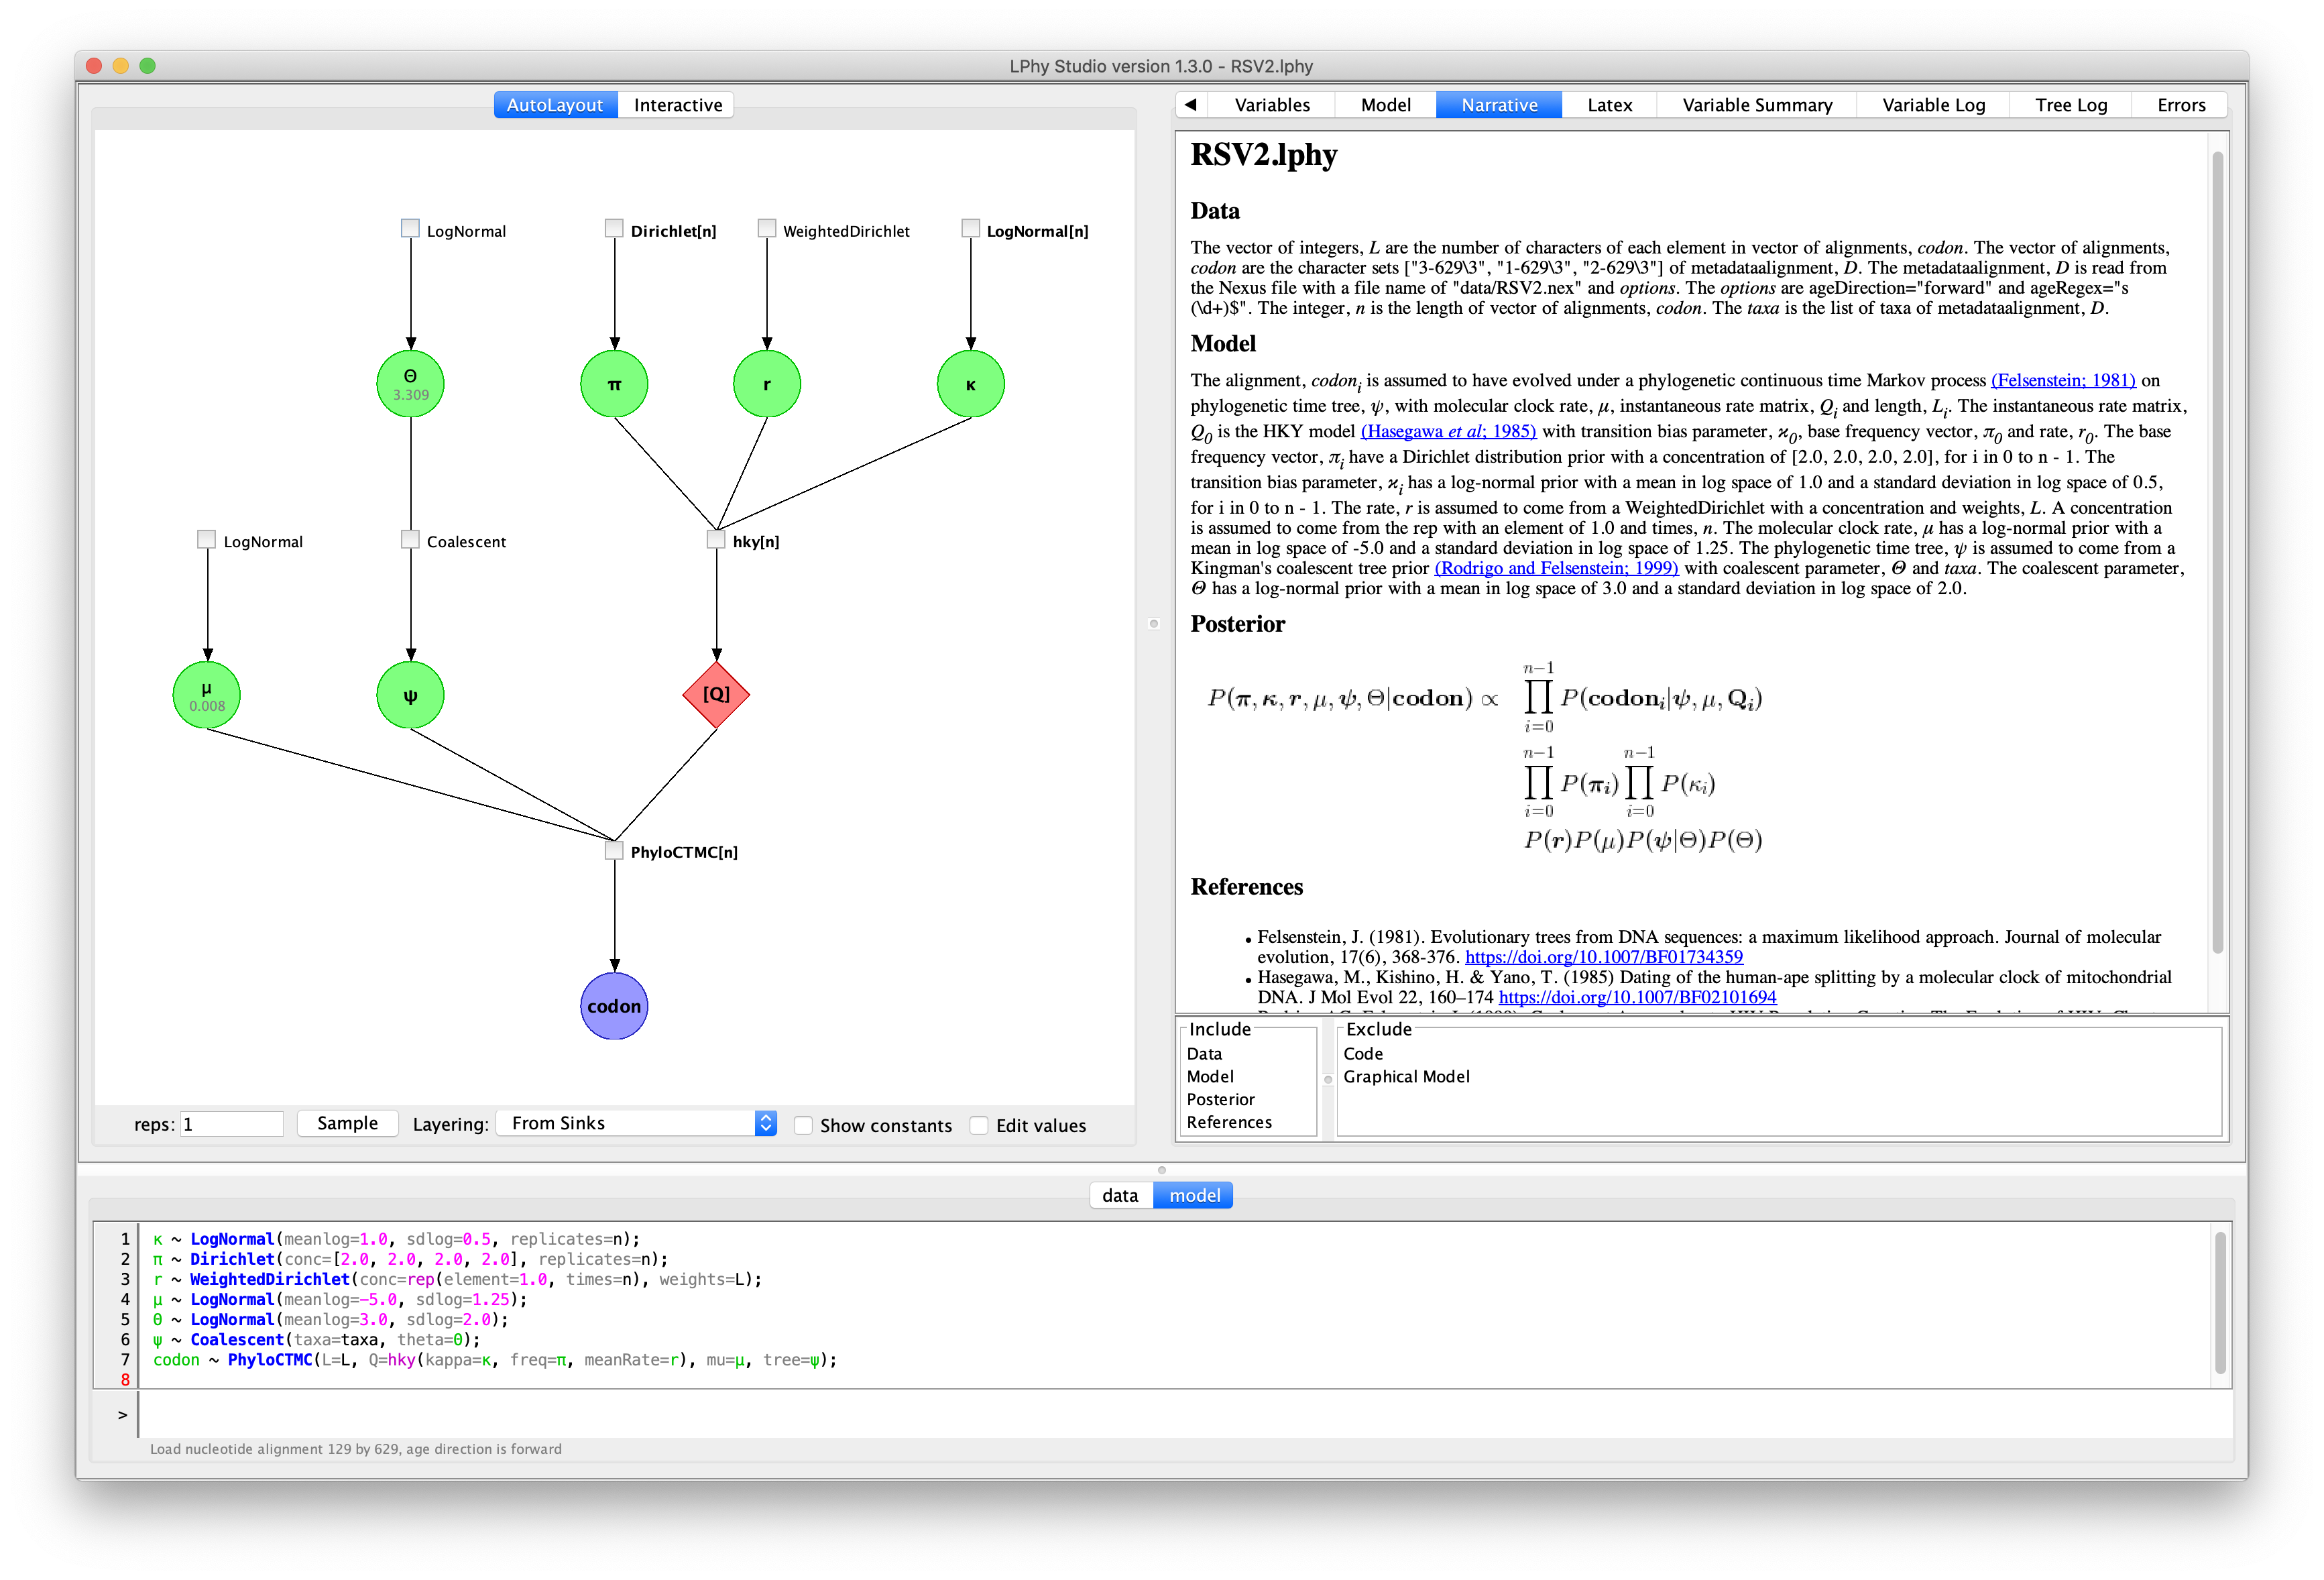
\includegraphics[width=\textwidth]{figs/lphystudio_screenshot.png}
  \caption{A screenshot of LPhy Studio showing the probabilistic graphical model 
  on the left panel (constants hidden), and the auto-generated text description of the data and phylogenetic model on the right panel.} 
  \label{fig:lphystudio}
\end{figure}

The GUI can either import the existing LPhy script or take the script typed from the console on the bottom of LPhy Studio panel. Either way the Studio will guarantee to produce the same graphical probability model representing the specified phylogenetic model. 
This allows the user focusing on a simple script while sharing the same visualizations across different collaborators.  

The narrative generator integrated with LPhyStudio can automatically create human-readable descriptions about the data, model, and posterior distribution. 
It also includes the mathematical definition of the posterior of the given model, and some relevant academic references regarding the model. 
The generator can also produce these contents in a Latex format, so that the user could simply copy them into a publication manuscript as the reference of the model applied. 
This will take most researchers in an easy way to precisely describe their models for publishing a Bayesian phylogenetic analysis. 


\subsection{A model guide for users}
There are two learning curves for a beginner level of users, one is to learn the LPhy language, the other is to understand the model. To shorten these learning curves, a tool with GUI, called Model Guide, is implemented to list all available LPhy generative distributions and functions in runtime. 
They are classified into several categories for users to look up easily.

Selecting a model or function, e.g. Figure \ref{fig:modelguide}, the user can find its usage, description, and the example scripts (they are accessible from LPhy Studio). For a published model, the citation is also provided for the convenience of learning, if it has DOI or book ISBN number, the hyperlink will lead the reader to the online publication.   

\textcolor{blue}{TODO: Figure to suppl?}

\begin{figure}
  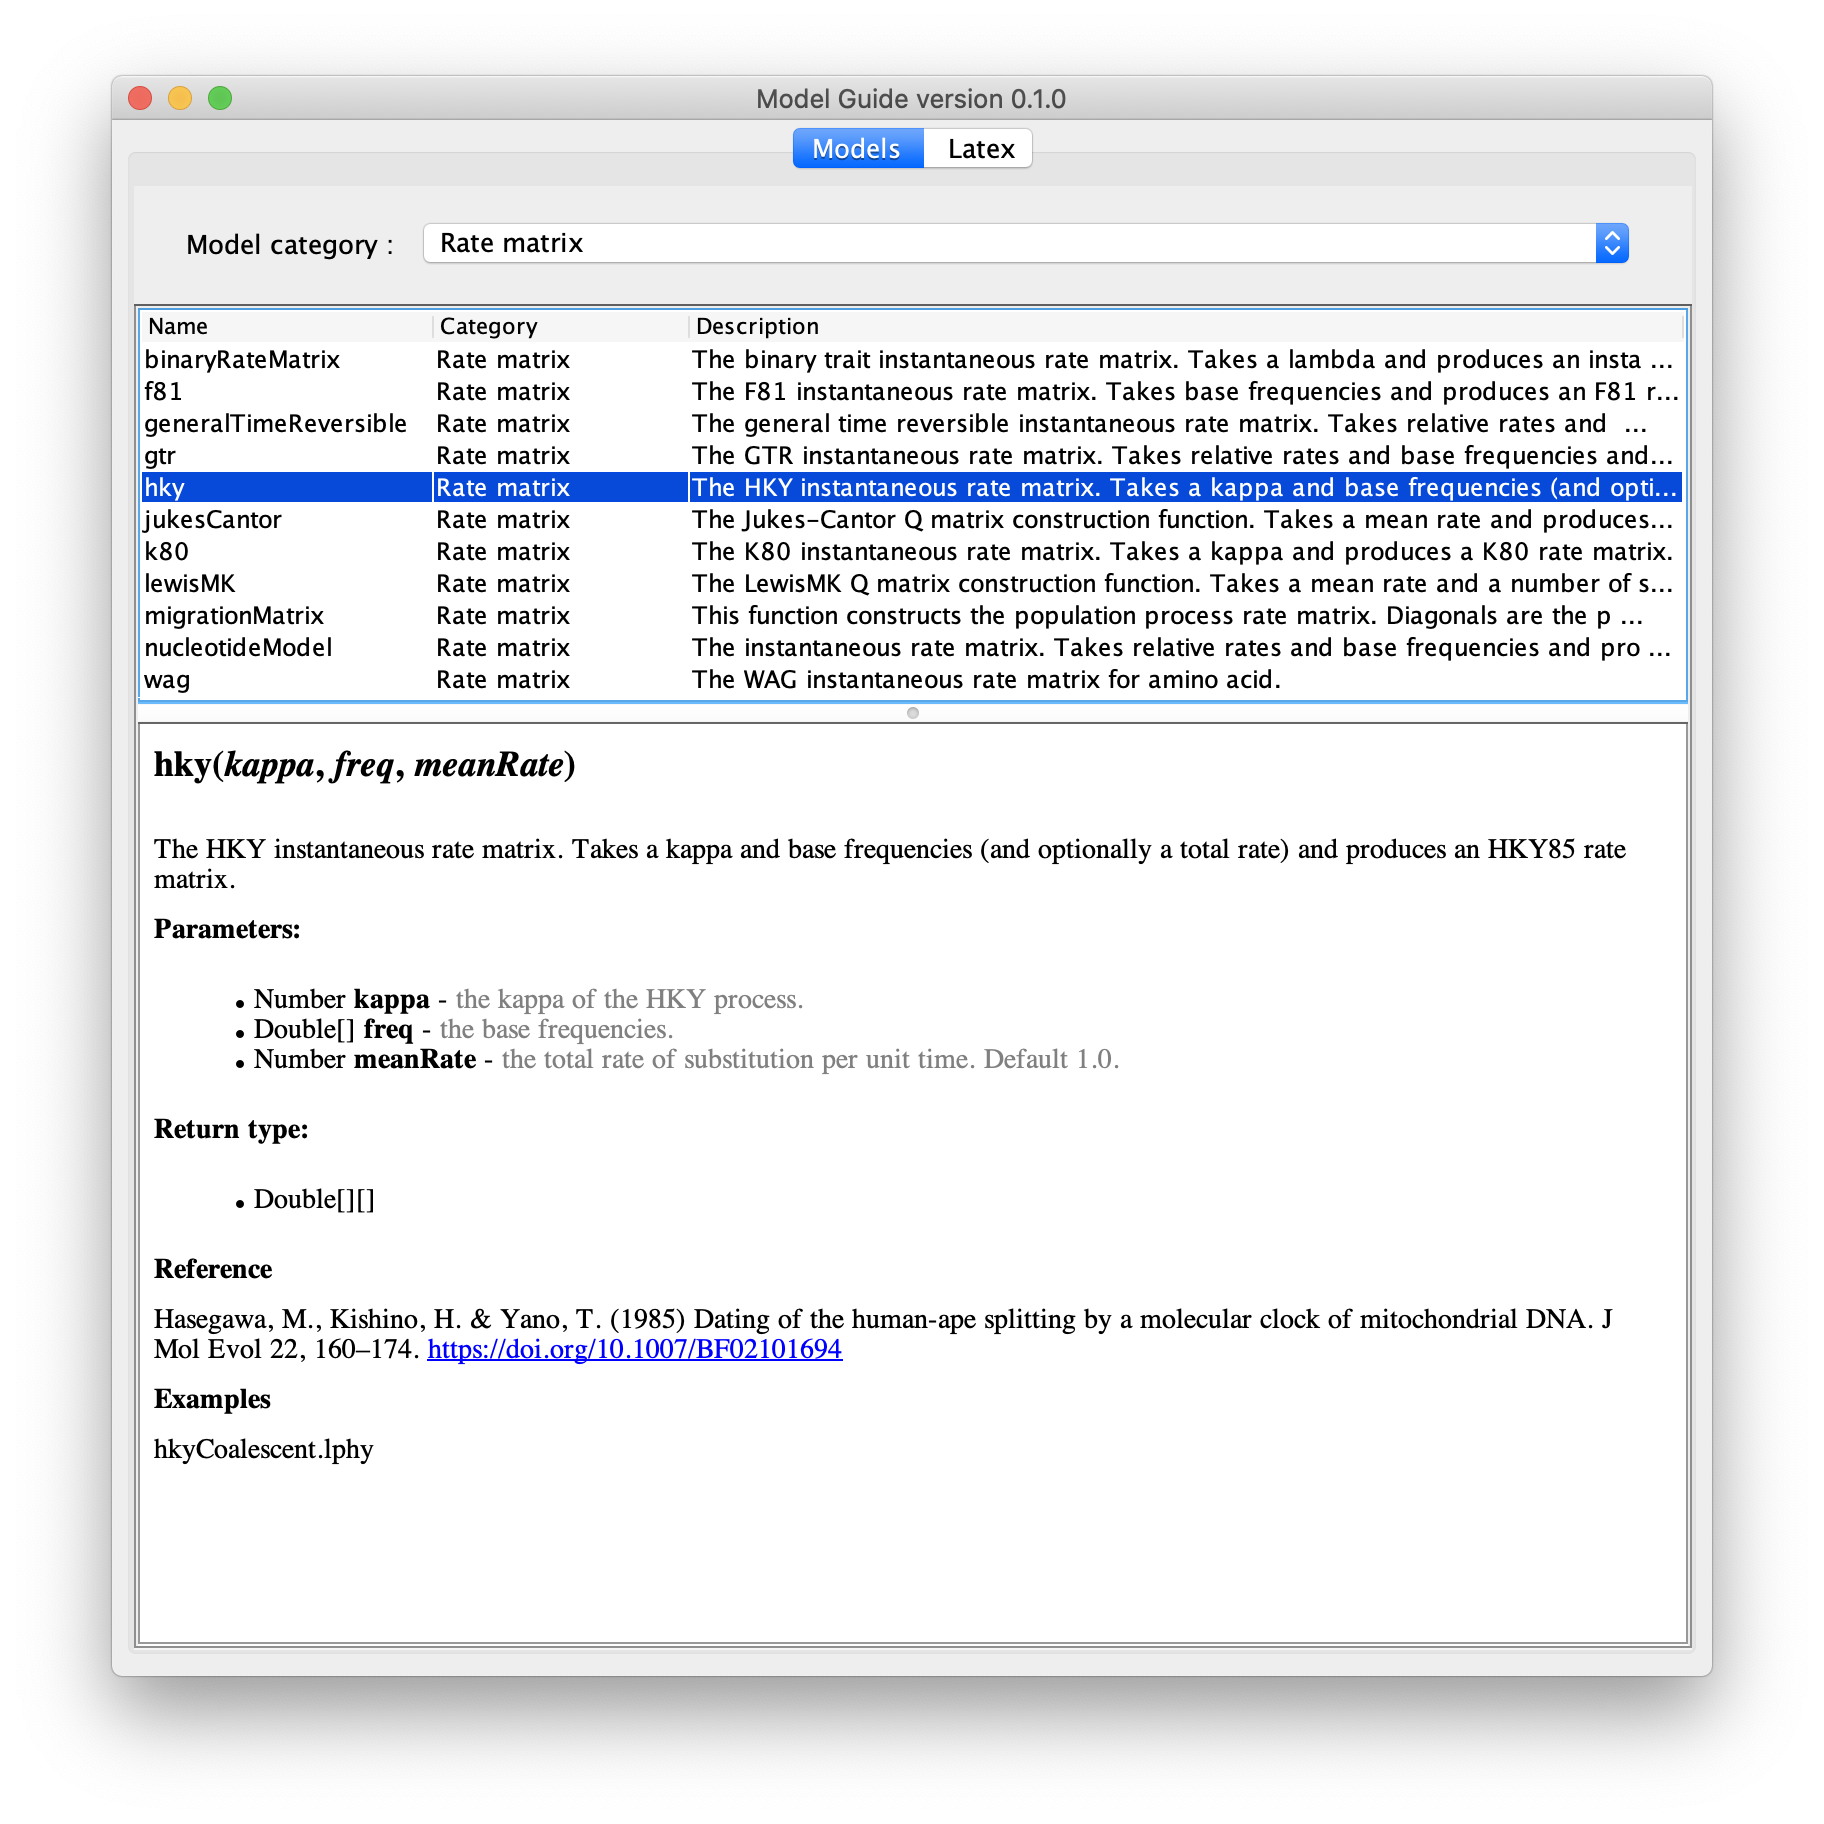
\includegraphics[width=\textwidth]{figs/modelguide.png}
  \caption{A screenshot of Model Guide showing the usage of \emph{hky} function, its example script, and the citation of HKY85 model.} 
  \label{fig:modelguide}
\end{figure}


\subsection{Data simulations from a phylogenetic model}
Simulating alignments from a specified model can ever be easy using the LPhy Studio. This can be simply done by loading a LPhy script and then clicking the ``Sample" button. 
It logs both ``true" values of the parameters and ``true" trees simulated from the specified model defined in the LPhy script. 
The result of running 100 simulations from the simple HKY+Coalescent model is illustrated in Figure \ref{fig:simulations100}. 

\textcolor{blue}{TODO: Figure to suppl?}

\begin{figure}
  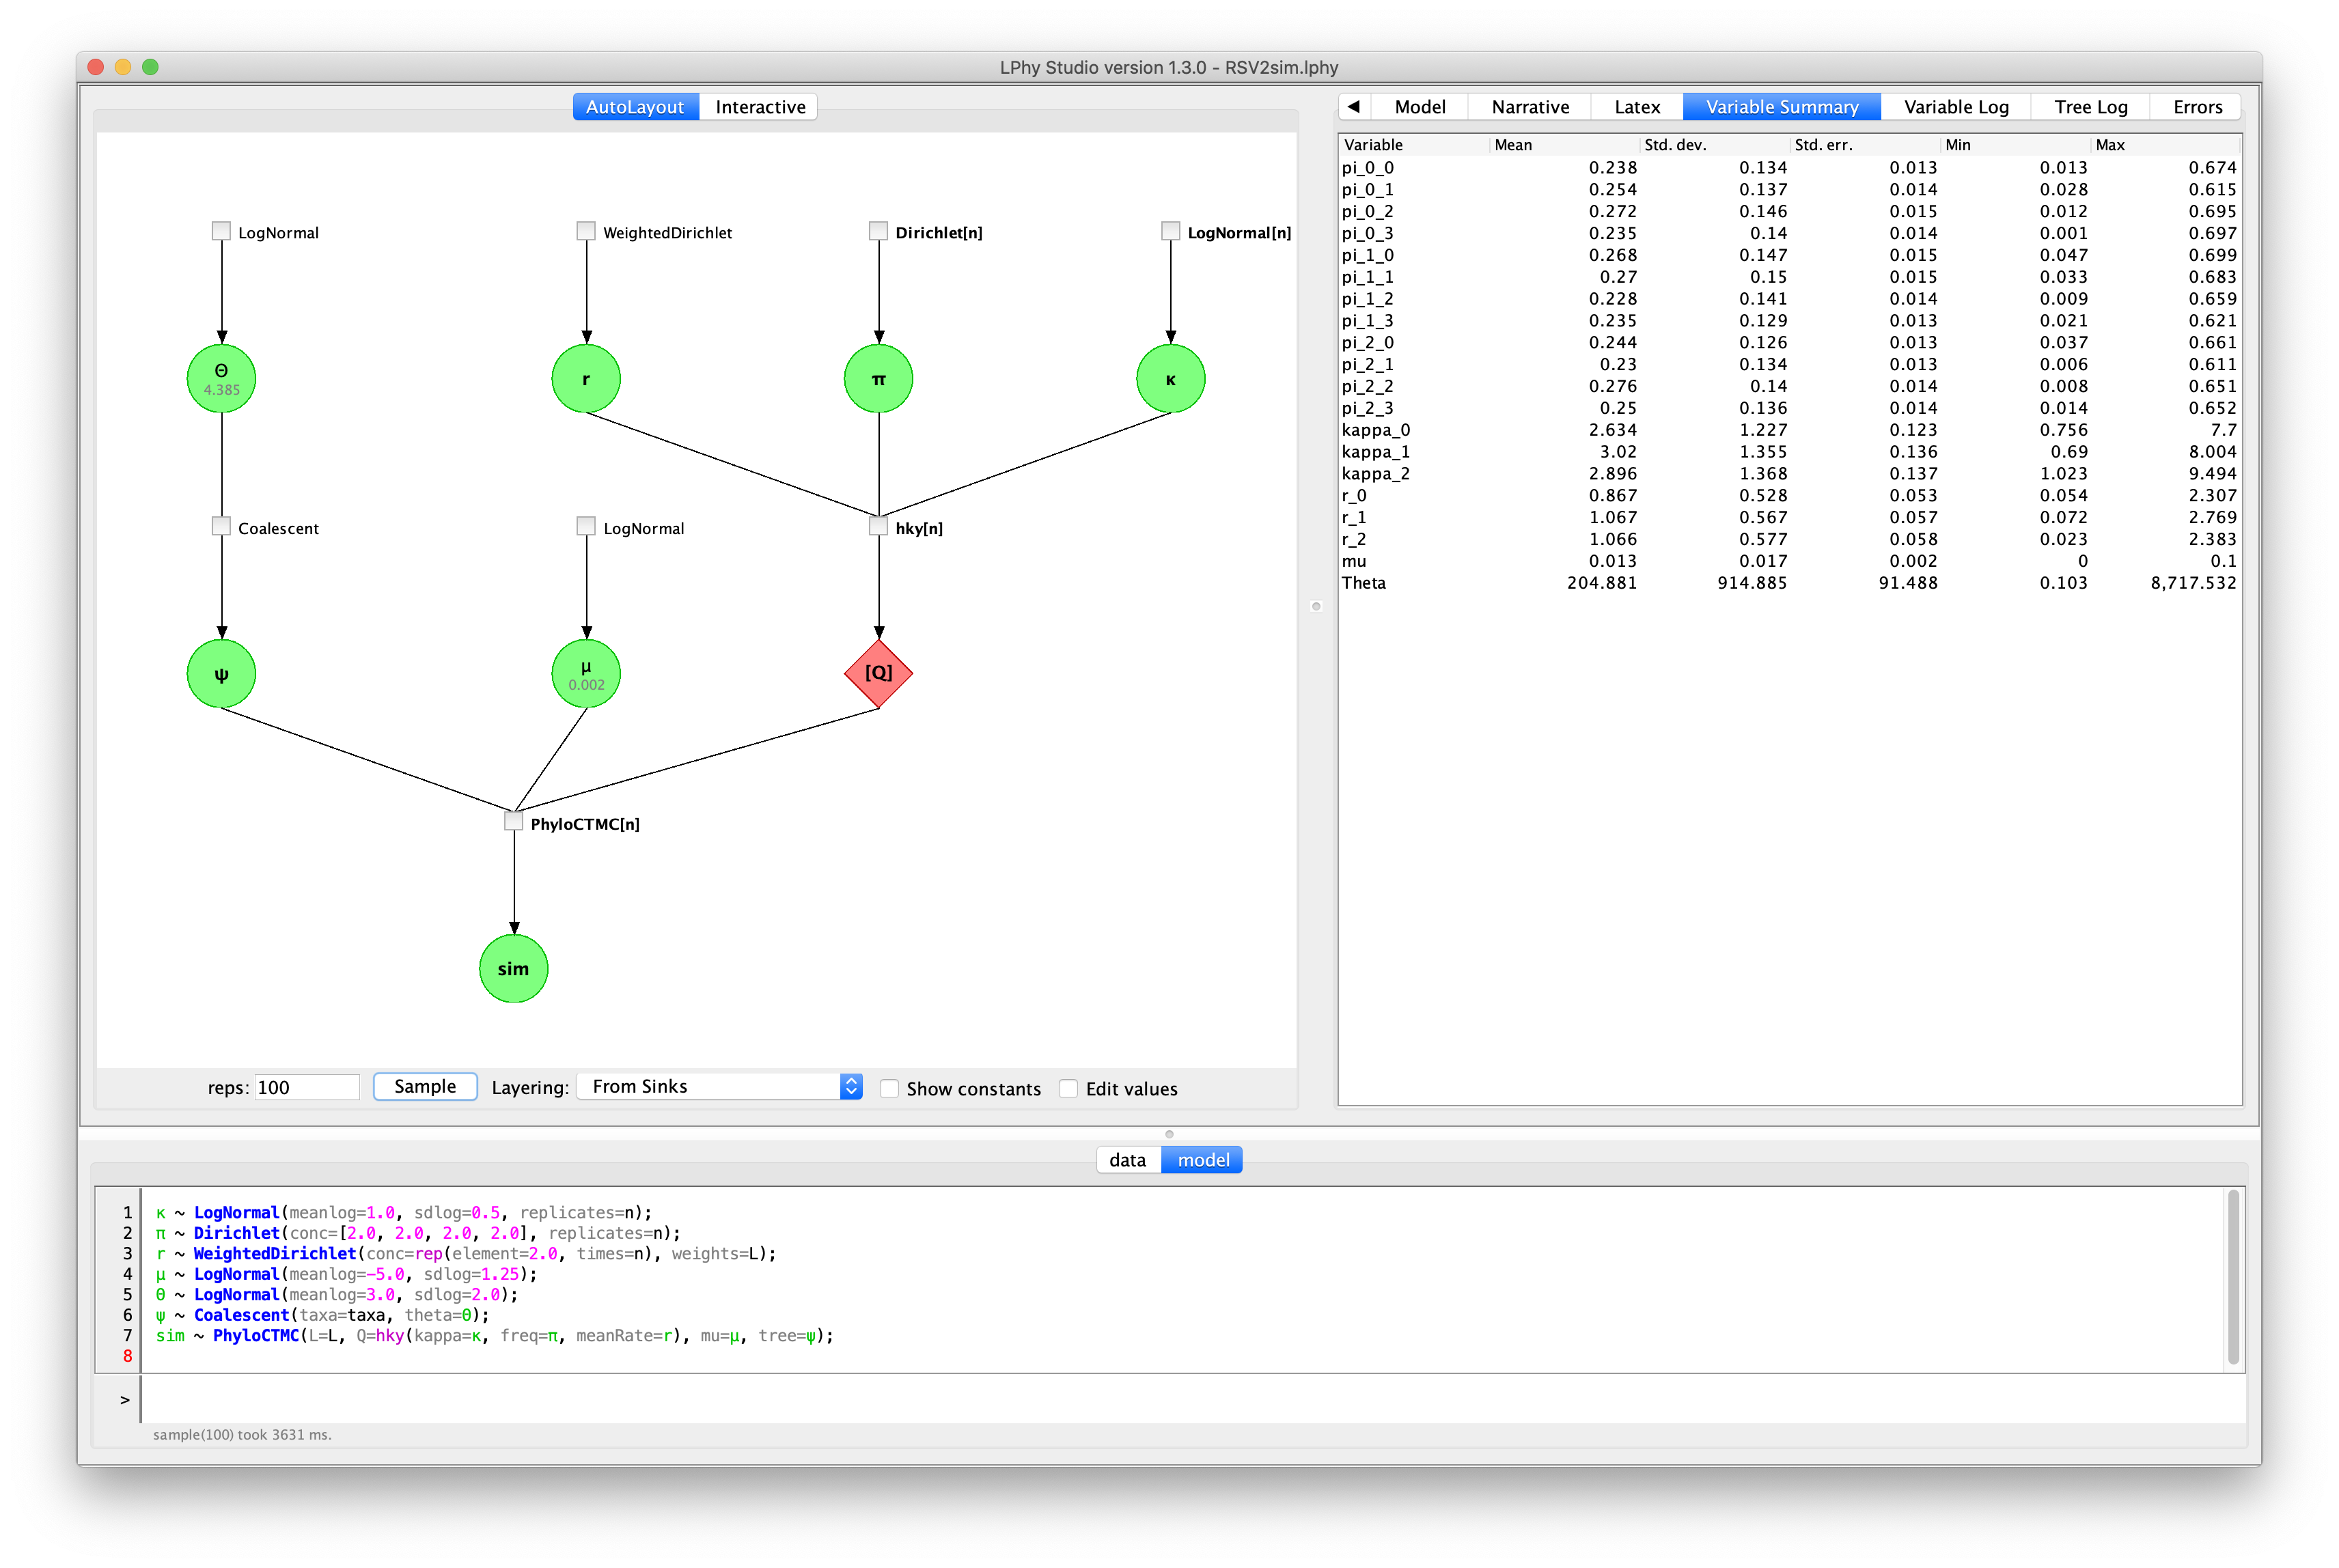
\includegraphics[width=\textwidth]{figs/simulations100.png}
  \caption{A screenshot to run 100 simulations from the simple HKY+Coalescent model. The ``reps'' text field is used to define the number of simulations to run. The right panel shows the statistical summary of the simulated parameters.} 
  \label{fig:simulations100}
\end{figure}


\subsection{Integration with Bayesian phylogenetic inference frameworks}
LPhy specifies the models, but we also provide an integration with BEAST2 \cite{bouckaert2014beastanalysis,bouckaert2019beastanalysis}, called as LPhyBEAST, for the models specified in the LPhy language to be applied to data using Bayesian inference.
It is a command-line program that takes a LPhy script file including model specification and data block, and then produces a BEAST2 XML file. 
It is therefore an alternative way to succinctly express and communicate BEAST2 analyses.

More Integrations are proposing to convert an LPhy specification into an input file that other popular Bayesian phylogenetic inference tools, such as BEAST1\cite{suchard2018bayesian}, MrBayes\cite{ronquist2012mrbayes}, RevBayes\cite{hohna2016revbayes}, etc., can understand.


\subsection{Model validation}
\textcolor{blue}{KC TODO}


\section*{Discussion and conclusions}
\textcolor{blue}{TODO}

Although there are many
programming languages through which statistical 
models can be succintly described (e.g., Stan
\cite{carpenter2017stan}, JAGS \cite{plummer2003jags}, BUGS
\cite{lunn2009bugs, gilks1994language}), these languages do not
support the unique feature of phylogenetic models: the phylogenetic
tree.
Phylogenetic trees are complex high-dimensional objects, part
discrete, part continuous.
% There is no bijection between tree space and Euclidean space, so these
% objects cannot be treated with standard statistical distributions
% \textcolor{red}{[Should you cite something here?]}.
Hence, specialist software is needed to perform inference
involving phylogenetic trees
\cite{hohna2016revbayes,bouckaert2019beastanalysis}.

...

LinguaPhylo is similar to the popular R language \cite{R} in that it
has built-in vectorization, meaning that any function (including
generative distributions) can be called with its arguments in
vectorized form, producing multiple values as its output. 


\section*{Acknowledgments}
Thanks for the New Zealand eScience Infrastructure (NeSI) to provide the high performance computation resource for our model validations.

\nolinenumbers

% Either type in your references using
% \begin{thebibliography}{}
% \bibitem{}
% Text
% \end{thebibliography}
%
% or
%
% Compile your BiBTeX database using our plos2015.bst
% style file and paste the contents of your .bbl file
% here. See http://journals.plos.org/plosone/s/latex for 
% step-by-step instructions.
% 
\bibliography{linguaPhylo}



\end{document}

